\documentclass[aspectratio=169]{beamer}
\usetheme{Madrid}

\usepackage[T1]{fontenc}
\usepackage[utf8]{inputenc}
\usepackage{amsmath,amssymb,physics,bm}
\usepackage{graphicx}
\usepackage{tikz}

\title{From PDEs to Chaos: The Lorenz System}
\author{PHYS 340 -- Methods of Theoretical Physics}
\date{Final Lecture}

\begin{document}

\frame{\titlepage}

\begin{frame}{Why End the Course Here?}
\begin{itemize}
\item Much of theoretical physics begins with a PDE.
\item PDEs usually describe systems with infinitely many degrees of freedom.
\item But often, the large-scale physics is captured by only a few dominant modes.
\item The Lorenz system is a famous example: a fluid PDE reduced to three coupled ODEs.
\item The result is not merely simpler mathematics --- it reveals chaos.
\end{itemize}
\end{frame}

\begin{frame}{The Big Question}
A natural question for this course is:

\vspace{0.5em}

\begin{center}
\Large
How can a field theory in space and time become a finite-dimensional dynamical system?
\end{center}

\vspace{0.8em}

Today's roadmap:
\begin{enumerate}
\item Start with thermal convection.
\item Expand the fields in spatial modes.
\item Truncate to a few dominant amplitudes.
\item Obtain a nonlinear system of ODEs.
\item Discover that simple deterministic equations can behave chaotically.
\end{enumerate}
\end{frame}

\begin{frame}{PDEs Versus ODEs}
\begin{columns}[T]
\column{0.48\textwidth}
\textbf{PDE viewpoint}
\begin{itemize}
\item Unknown depends on space and time
\item Example: $u(x,z,t)$
\item Need boundary conditions
\item Usually infinitely many modes
\end{itemize}

\column{0.48\textwidth}
\textbf{ODE viewpoint}
\begin{itemize}
\item Unknown depends only on time
\item Example: $x(t)$, $y(t)$, $z(t)$
\item Finite-dimensional phase space
\item Easier to analyze geometrically
\end{itemize}
\end{columns}

\vspace{0.8em}

The Lorenz model is the bridge between these two viewpoints.
\end{frame}

\begin{frame}{Rayleigh--B\'enard Convection}
A shallow fluid layer is heated from below and cooled from above.  The goal here is to determine: $T(x,z,t)$, $p(x,z,t)$, $\vec{v}(x,z,t)$

\begin{center}
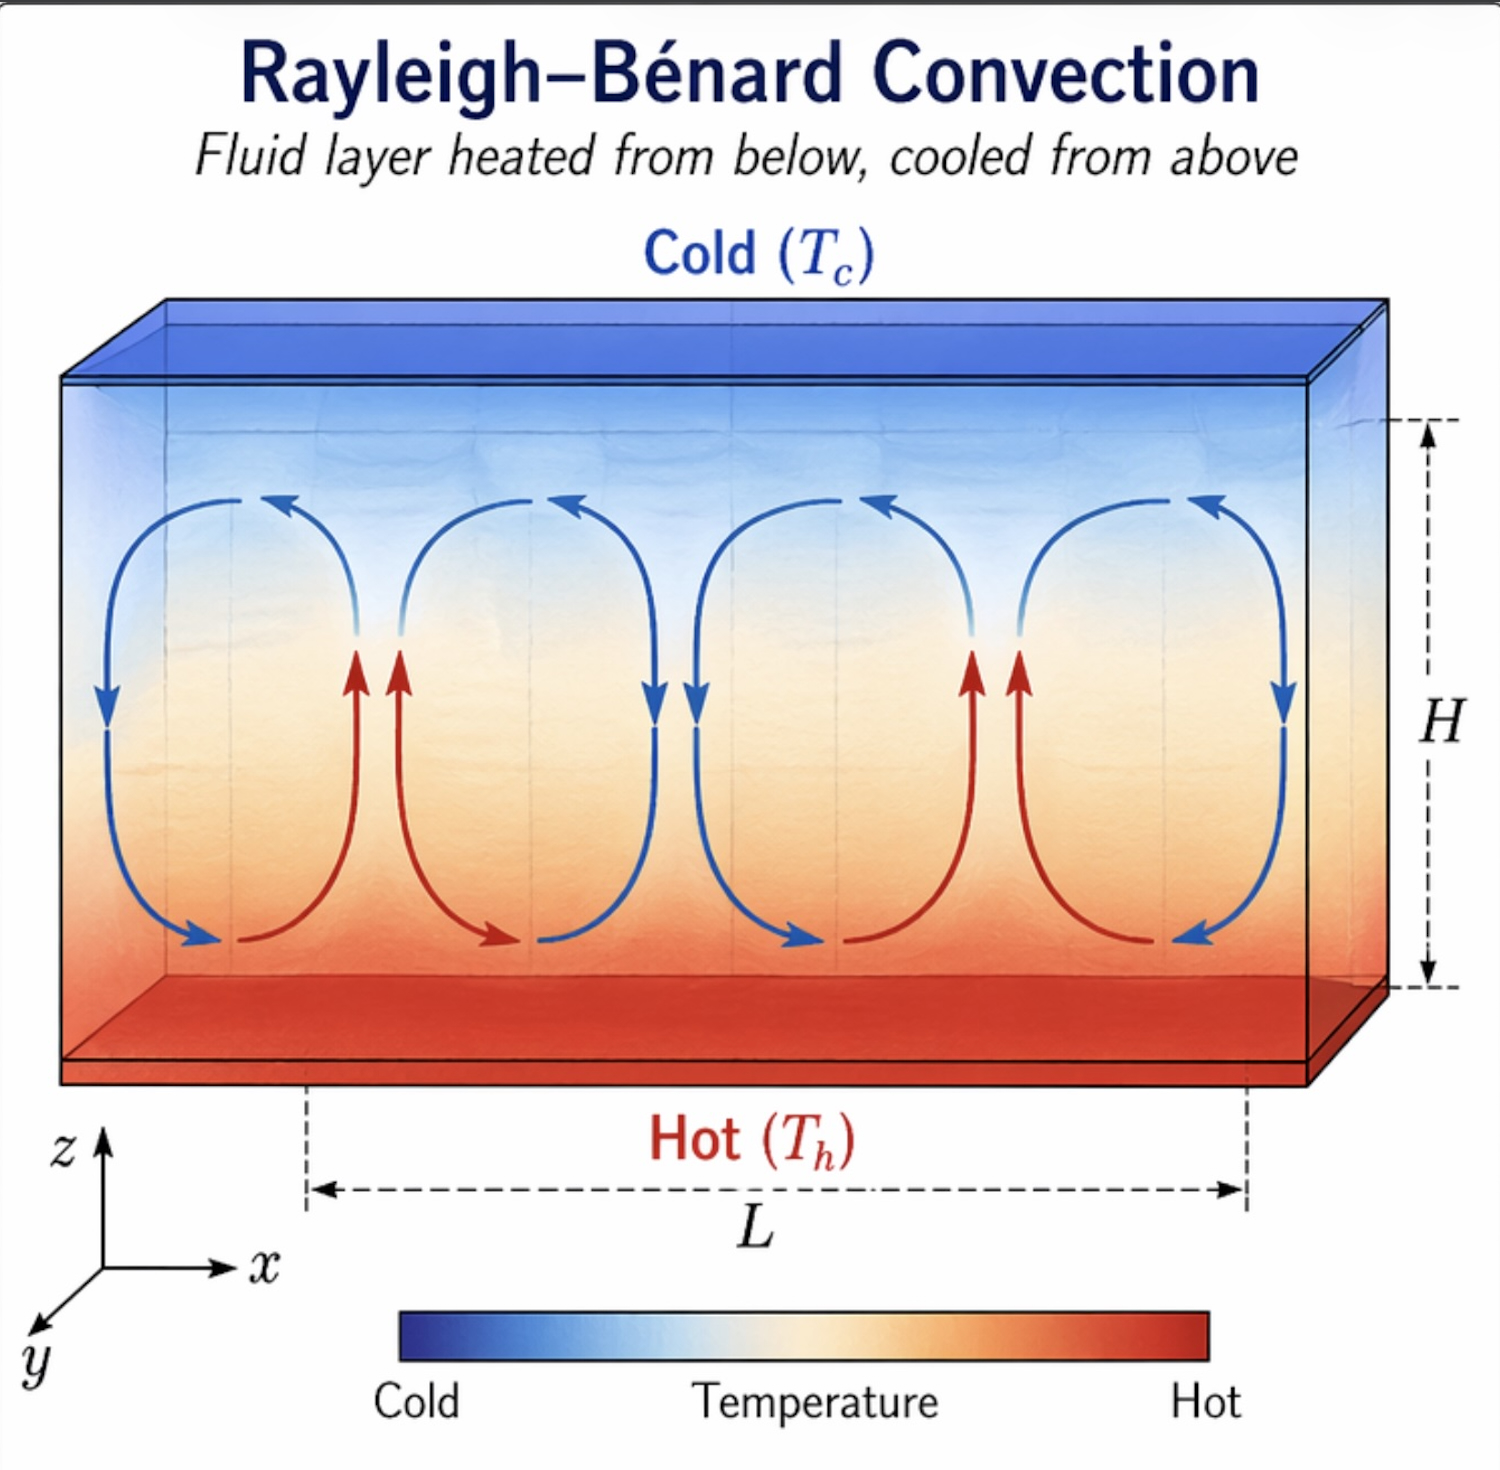
\includegraphics[height=0.72\textheight]{convection_placeholder.jpg}
\end{center}
\end{frame}

\begin{frame}{Physical Picture of the Instability}
\begin{itemize}
\item If the temperature difference is small, heat is carried mainly by conduction.
\item A fluid parcel that rises enters a region of lower pressure and can remain warmer than its surroundings.
\item Warm fluid is less dense, so buoyancy pushes it upward further.
\item Likewise, cooler fluid can sink.
\item But, \textbf{beyond a critical threshold}, the conduction state becomes unstable and convection rolls appear.
\end{itemize}

\vspace{1em}
\center
\textbf{This is an instability problem --- a central theme of theoretical physics!}
\end{frame}

\begin{frame}{Why the Governing Equations Are PDEs}
The state of the fluid depends on position and time:
\begin{itemize}
\item velocity field $\vec{\vb{v}}(x,z,t)$
\item temperature field $T(x,z,t)$
\item pressure field $p(x,z,t)$
\end{itemize}

So the dynamics involve derivatives such as
\begin{equation*}
\pdv{T}{t}, \qquad \pdv{T}{x}, \qquad \pdv[2]{T}{z}, \qquad \pdv{\vb{v_x}}{t}, \qquad \pdv{\vb{v_z}}{x}, \qquad \pdv{\vb{p}}{z}
\end{equation*}
and therefore the equations are PDEs.

\vspace{0.5em}

We will not derive the full fluid equations today; our focus is the \textbf{method of reduction}.
\end{frame}

\begin{frame}{The Mathematical Strategy}
This lecture uses a pattern that appears all over PHYS 340:
\begin{enumerate}
\item Choose basis functions that respect the geometry and boundaries.
\item Expand the unknown fields in those basis functions.
\item Substitute the expansion into the PDEs.
\item Use orthogonality to project onto selected modes.
\item Obtain ODEs for the mode amplitudes.
\item Truncate to the most important modes.
\end{enumerate}

\begin{center}
\Large
Expand $\rightarrow$ Project $\rightarrow$ Truncate $\rightarrow$ Analyze
\end{center}
\end{frame}

\begin{frame}{Mode Expansions: The General Idea}
Suppose a field depends on space and time:
\begin{equation*}
u(x,z,t)
\end{equation*}
Write it as a sum of spatial patterns with time-dependent amplitudes:
\begin{equation*}
u(x,z,t)=\sum_{m,n} a_{mn}(t)\,\phi_{mn}(x,z)
\end{equation*}

Interpretation:
\begin{itemize}
\item $\phi_{mn}(x,z)$ describes a spatial shape or pattern.
\item $a_{mn}(t)$ tells us how strongly that pattern is excited at time $t$.
\end{itemize}

This is the same basic philosophy as Fourier series, normal modes, and eigenfunction expansions.
\end{frame}

\begin{frame}{Why Sines and Cosines?}
For rectangular geometry and simple boundary conditions, trigonometric modes are natural:
\begin{equation*}
\sin\!\left(\frac{m\pi x}{L}\right), \qquad
\cos\!\left(\frac{m\pi x}{L}\right), \qquad
\sin\!\left(\frac{n\pi z}{H}\right)
\end{equation*}

Why they are useful:
\begin{itemize}
\item They often satisfy the boundary conditions automatically.
\item They are orthogonal on the domain.
\item They are ordered from large-scale to fine-scale structure.
\item They turn PDEs into algebraic coupling between amplitudes.
\end{itemize}
\end{frame}

\begin{frame}{Orthogonality Is the Key Step}
If the basis functions are orthogonal, then different modes separate cleanly.

Schematically,
\begin{equation*}
\int \phi_m(x,z)\,\phi_n(x,z)\,dV = 0
\qquad (m \neq n)
\end{equation*}

That means when we multiply the PDE by a chosen basis function and integrate, we isolate the equation for that mode.

\vspace{0.5em}

This is a Galerkin-style projection method.
\end{frame}

\begin{frame}{A Sketch of the Convection Expansion}
Edward Lorenz (1963 - Atmostpheric Convection) kept only a few carefully chosen large-scale modes.
For example, one may write the streamfunction (like electric potential!) and temperature perturbation ($T - T_0$) schematically as
\begin{equation*}
\psi(x,z,t)=X(t)\sin\!\left(\frac{\pi a x}{H}\right)\sin\!\left(\frac{\pi z}{H}\right)
\end{equation*}
and
\begin{equation*}
\theta(x,z,t)=Y(t)\cos\!\left(\frac{\pi a x}{H}\right)\sin\!\left(\frac{\pi z}{H}\right)
- Z(t)\sin\!\left(\frac{2\pi z}{H}\right)
\end{equation*}

The exact form is less important today than the idea:
\begin{center}
\large
a small number of spatial modes $\Rightarrow$ a small number of amplitudes.
\end{center}
\end{frame}

\begin{frame}{What Is the Streamfunction?}
For two-dimensional incompressible flow, write the velocity field as
\begin{equation*}
\vec{\vb{v}}(x,z,t) = \bigl(u(x,z,t),\,w(x,z,t)\bigr).
\end{equation*}

Incompressibility ($\vec{\nabla} \cdot \vec{\vb{v}} = 0$) requires
\begin{equation*}
\pdv{u}{x} + \pdv{w}{z} = 0.
\end{equation*}

A convenient way to satisfy this automatically is to introduce the
\textbf{streamfunction} $\psi(x,z,t)$, defined by
\begin{equation*}
u = \pdv{\psi}{z},
\qquad
w = -\pdv{\psi}{x}.
\end{equation*}

Then
\begin{equation*}
\pdv{u}{x} + \pdv{w}{z}
=
\pdv{}{x}\left(\pdv{\psi}{z}\right)
-
\pdv{}{z}\left(\pdv{\psi}{x}\right)
=0.
\end{equation*}

So $\psi$ encodes the fluid motion, and its amplitude measures the strength
of the circulating convection roll.
\end{frame}

\begin{frame}{What Is the Temperature Perturbation?}
Write the total temperature field as
\begin{equation*}
T(x,z,t)=T_{\text{base}}(z)+\theta(x,z,t).
\end{equation*}

Here:
\begin{itemize}
\item $T_{\text{base}}(z)$ is the static conduction profile, depending only on height.
\item $\theta(x,z,t)$ is the \textbf{temperature perturbation}, the departure from that simple linear profile.
\end{itemize}

Physically, $\theta$ describes the thermal structure created by convection:
\begin{itemize}
\item warm fluid rising,
\item cool fluid sinking,
\item horizontal temperature differences across a convection cell,
\item distortion of the vertical temperature gradient.
\end{itemize}

In the Lorenz truncation:
\begin{itemize}
\item $X(t)$ measures the strength of the flow pattern,
\item $Y(t)$ measures the horizontal temperature contrast,
\item $Z(t)$ measures distortion of the vertical temperature profile.
\end{itemize}
\end{frame}

\begin{frame}{What Happens Before Truncation?}
If we keep \emph{all} modes, then substituting the expansion into the PDEs gives:
\begin{itemize}
\item an infinite set of coupled ODEs for the amplitudes
\item linear terms from diffusion or damping
\item nonlinear coupling terms from advection
\end{itemize}

So the PDE has not magically disappeared --- it has been rewritten as an infinite dynamical system.  

If we do not truncate, we are dealing with the full infinite-dimensional fluid PDE rather than a toy model. That places us back in the realm of Navier–Stokes-type dynamics, where some of the deepest open problems in mathematics still live.

\vspace{0.5em}
\center
\textbf{The drastic approximation is to keep only the most important amplitudes}
\end{frame}

\begin{frame}{Why Truncation Can Work}
Why is it even reasonable to keep only a few modes?
\begin{itemize}
\item Near the onset of instability, only a few large-scale modes are unstable.
\item Higher spatial frequencies are often strongly damped.
\item The large-scale qualitative behavior can be controlled by low-order structure.
\item A reduced model may capture the essential mechanism even if it misses fine detail.
\end{itemize}

This is one of the deepest lessons of mathematical physics:
\begin{center}
\large
\textbf{approximation is not the enemy of understanding.}
\end{center}
\end{frame}

\begin{frame}{The Lorenz Truncation}
Lorenz reduced the dynamics to three time-dependent amplitudes:
\begin{equation*}
X(t), \qquad Y(t), \qquad Z(t)
\end{equation*}

After rescaling variables and parameters, the resulting equations are
\begin{align*}
\dot{x} &= \sigma(y-x), \\
\dot{y} &= rx-y-xz, \\
\dot{z} &= xy-bz.
\end{align*}

This is the Lorenz system.
\end{frame}

\begin{frame}{How Do We Recover $X$, $Y$, and $Z$?}
The variables $X,Y,Z$ are coefficients in a mode expansion.

If
\begin{equation*}
\psi(x,z,t)=X(t)\phi_1(x,z),
\end{equation*}
then orthogonality gives
\begin{equation*}
X(t)=
\frac{\int \psi(x,z,t)\,\phi_1(x,z)\,dV}
{\int \phi_1^2(x,z)\,dV}.
\end{equation*}

Likewise,
\begin{equation*}
Y(t)=
\frac{\int \theta(x,z,t)\,\phi_2(x,z)\,dV}
{\int \phi_2^2(x,z)\,dV},
\qquad
Z(t)=
\frac{\int \theta(x,z,t)\,\phi_3(x,z)\,dV}
{\int \phi_3^2(x,z)\,dV}.
\end{equation*}

So $X,Y,Z$ are generalized coordinates obtained by projection onto chosen spatial modes.
\end{frame}

\begin{frame}{What Do the Variables Mean?}
The variables are not particle positions. They are mode amplitudes.

\begin{itemize}
\item $x(t)$: strength of the convective circulation
\item $y(t)$: horizontal temperature contrast
\item $z(t)$: vertical distortion of the temperature profile
\end{itemize}

So the state of the reduced system is a point in a three-dimensional phase space.
\end{frame}

\begin{frame}{Linear Terms and Nonlinear Terms}
Look at the structure carefully:
\begin{align*}
\dot{x} &= \sigma(y-x), \\
\dot{y} &= rx-y-xz, \\
\dot{z} &= xy-bz.
\end{align*}

\begin{itemize}
\item Terms like $-x$, $-y$, and $-bz$ act like damping.
\item The term $rx$ represents driving controlled by the heating parameter $r$.
\item The products $xz$ and $xy$ are nonlinear couplings.
\end{itemize}

Those nonlinear couplings are what make the system qualitatively richer than a linear stability problem.
\end{frame}

\begin{frame}{Matrix Form of the Lorenz System}
Let
\begin{equation*}
\mathbf{u}(t)=
\begin{pmatrix}
x(t)\\[0.3em]
y(t)\\[0.3em]
z(t)
\end{pmatrix}.
\end{equation*}

Then the Lorenz equations can be written as
\begin{equation*}
\dot{\mathbf{u}}
=
\begin{pmatrix}
-\textcolor{red}{\sigma} & \textcolor{red}{\sigma} & 0\\[0.3em]
\textcolor{red}{r} & -1 & 0\\[0.3em]
0 & 0 & -\textcolor{red}{b}
\end{pmatrix}
\mathbf{u}
+
\begin{pmatrix}
0\\[0.3em]
-xz\\[0.3em]
xy
\end{pmatrix}.
\end{equation*}

\vspace{0.5em}

So the Lorenz system is:
\begin{itemize}
\item a \textbf{linear matrix system} controlled by
$\textcolor{red}{\sigma}$, $\textcolor{red}{r}$, and $\textcolor{red}{b}$,
\item plus a \textbf{nonlinear coupling term}.
\end{itemize}

Near an equilibrium point, the linear part is what connects to the eigenvalue/eigenvector analysis we studied earlier.
\end{frame}

\begin{frame}{Equilibria of the Lorenz System}
Set
\begin{equation*}
\dot{x}=\dot{y}=\dot{z}=0.
\end{equation*}

One obvious equilibrium is
\begin{equation*}
(x,y,z)=(0,0,0),
\end{equation*}
which corresponds roughly to no convective circulation.

For sufficiently large $r$, two additional equilibria appear:
\begin{equation*}
(x,y,z)=\left(\pm\sqrt{b(r-1)},\;\pm\sqrt{b(r-1)},\;r-1\right).
\end{equation*}

So even the steady-state structure already changes with parameter values.
\end{frame}

\begin{frame}{What Do the Parameters Mean Physically?}

Recall the Lorenz equations:
\begin{align*}
\dot{x} &= \sigma (y-x),\\
\dot{y} &= rx-y-xz,\\
\dot{z} &= xy-bz.
\end{align*}

The constants $\sigma$, $r$, and $b$ encode the physics of the fluid system:

\begin{itemize}
\item $\mathbf{r}$: the \textbf{heating strength}

Large $r$ means a larger temperature difference between the hot bottom plate and cold top plate.  
Increasing $r$ drives stronger convection.

\vspace{0.5em}

\item $\mathbf{\sigma}$: the ratio of momentum response to thermal response

It compares how quickly the fluid velocity adjusts versus how quickly heat diffuses

\vspace{0.5em}

\item $\mathbf{b}$: a geometric damping factor

It depends on the shape of the convection cells and controls how strongly the $z$-variable relaxes.

\end{itemize}

\vspace{0.5em}

So changing the parameters means changing the fluid, the geometry, or the heating.
\end{frame}

\begin{frame}{From Conduction to Chaos}

\begin{columns}[T]

\column{0.48\textwidth}
\centering
\textbf{Stable Conduction}

\vspace{0.3em}

$\sigma=10,\quad r=0.5,\quad b=\frac83$

\vspace{0.3em}

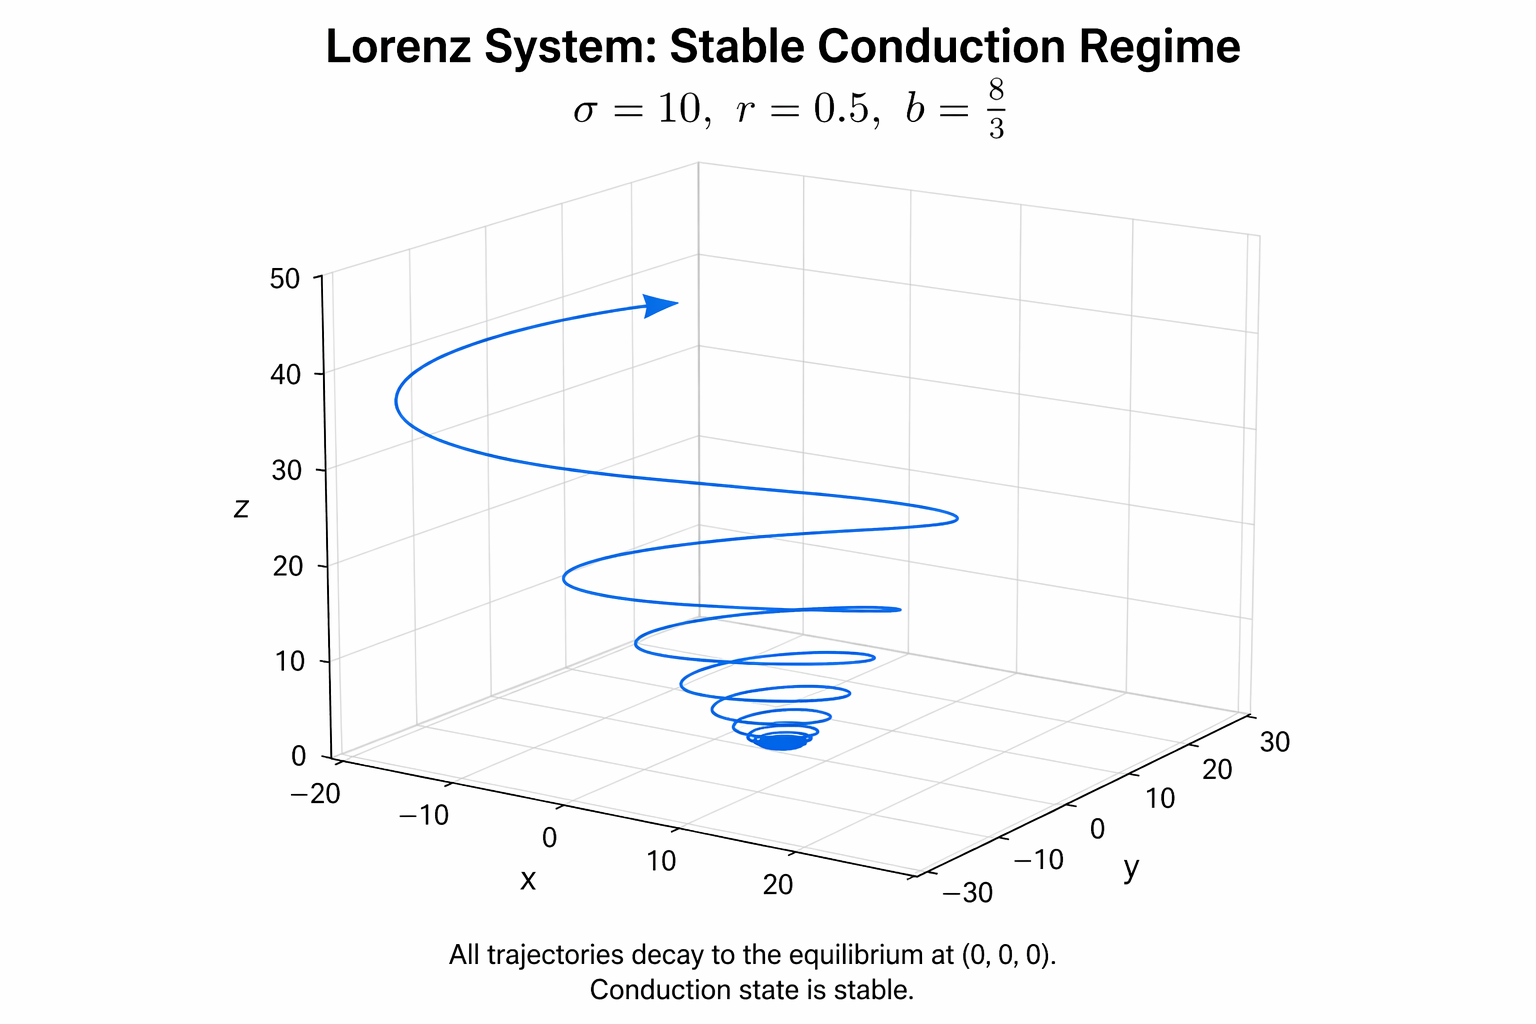
\includegraphics[height=0.55\textheight]{lorenz_stable.png}

Trajectories decay to the equilibrium state.

\column{0.48\textwidth}
\centering
\textbf{Chaotic Convection}

\vspace{0.3em}

$\sigma=10,\quad r=28,\quad b=\frac83$

\vspace{0.3em}

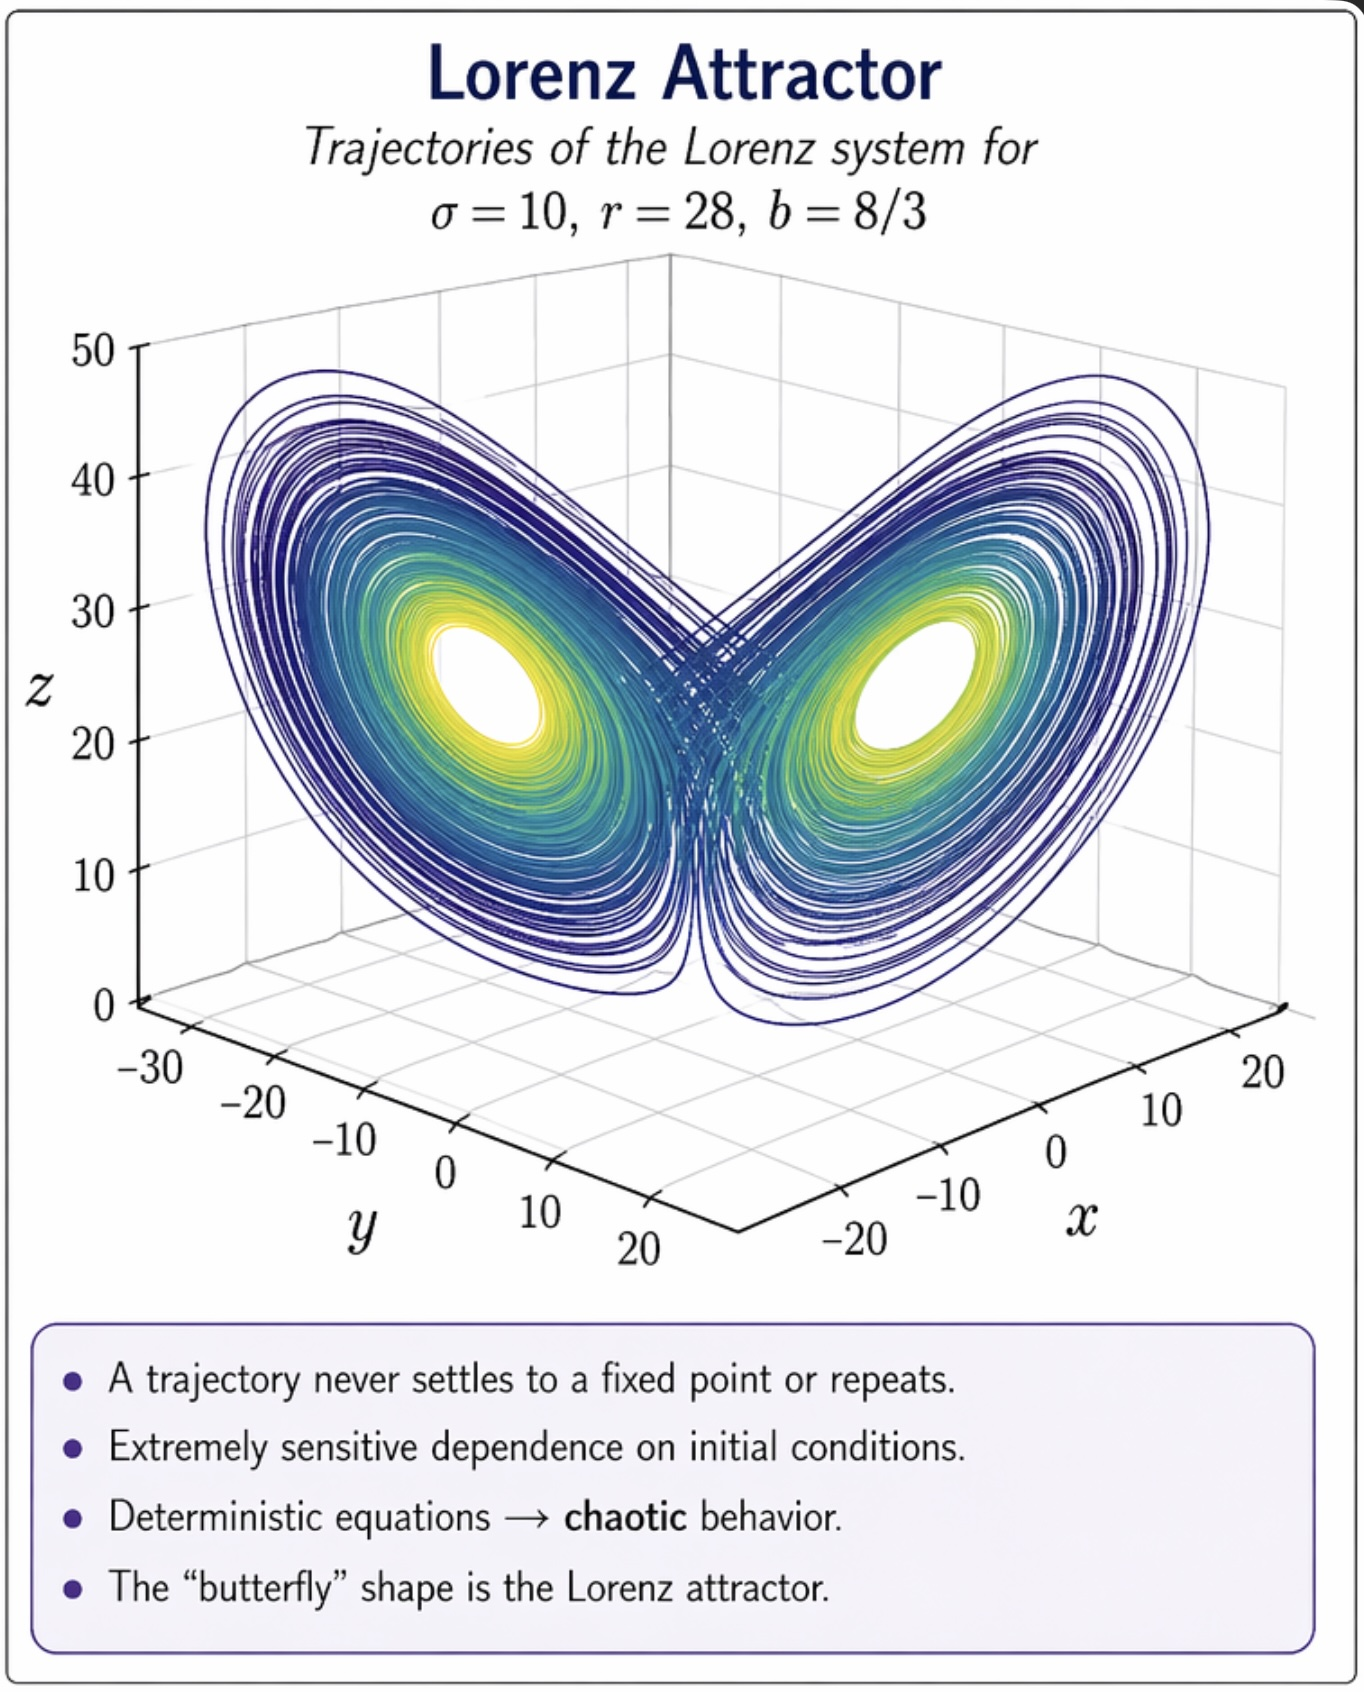
\includegraphics[height=0.55\textheight]{lorenz_placeholder.png}

Persistent motion on the strange attractor.

\end{columns}

\end{frame}


\begin{frame}{From Stability to Chaos}
For some parameter ranges, trajectories approach a fixed point.

For the classic parameter set
\begin{equation*}
\sigma=10, \qquad r=28, \qquad b=\frac{8}{3}
\end{equation*}
trajectories do something far more interesting:
\begin{itemize}
\item they do not settle to a steady state
\item they do not approach a simple periodic orbit
\item they keep wandering forever in a bounded region of phase space
\end{itemize}
\end{frame}

\begin{frame}{The Lorenz Attractor}
\begin{center}
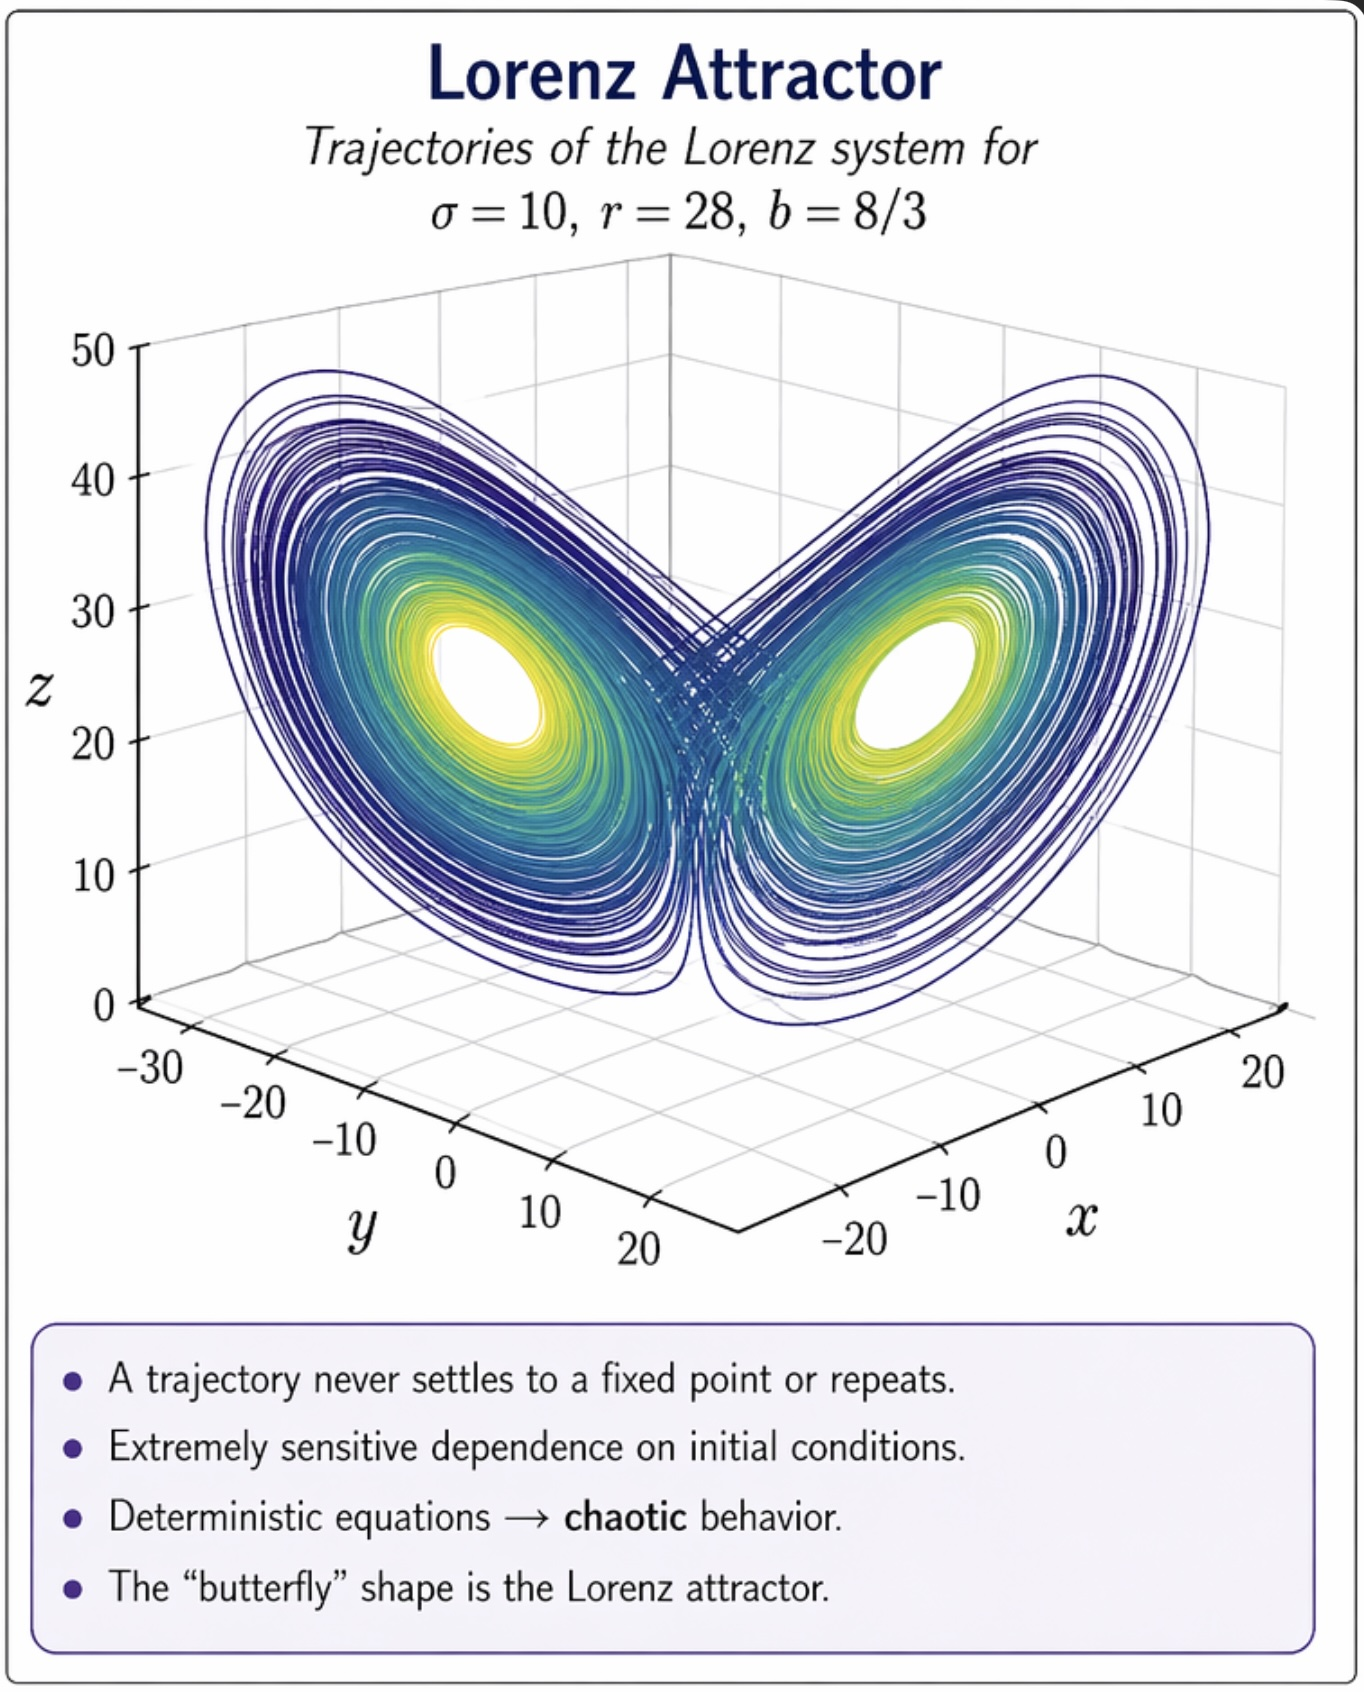
\includegraphics[height=0.9\textheight]{lorenz_placeholder.png}
\end{center}
\end{frame}

\begin{frame}{What Makes This So Striking?}
This system has only
\begin{itemize}
\item three variables
\item smooth deterministic equations
\item no random forcing
\end{itemize}

And yet the long-term motion is irregular and effectively unpredictable.

\vspace{0.8em}

This was historically shocking because it challenged the intuition that deterministic laws automatically imply long-term predictability.
\end{frame}

\begin{frame}{Sensitive Dependence on Initial Conditions}
Suppose two initial conditions differ by only a tiny amount.

In a chaotic regime:
\begin{itemize}
\item the two trajectories remain close only for a limited time
\item then they separate dramatically
\item long-term prediction becomes practically impossible
\end{itemize}

This is the mathematical content behind the phrase \emph{the butterfly effect}.
\end{frame}

\begin{frame}{What the Lorenz Model Does \emph{Not} Mean}
Important caution:
\begin{itemize}
\item Chaos is \textbf{not} the same as randomness.
\item The system is still completely deterministic.
\item If you know the exact initial condition, the future is uniquely determined.
\item The problem is that tiny uncertainty in initial data gets amplified.
\end{itemize}

So the issue is not absence of law --- it is extreme sensitivity within lawful dynamics.
\end{frame}

\begin{frame}{Why This Fits PHYS 340 So Well}
This example brings together many methods from the course:
\begin{itemize}
\item PDEs and boundary conditions
\item separation into spatial modes
\item orthogonality and projection
\item infinite series expansions
\item approximation and truncation
\item nonlinear ODE systems
\item equilibrium and stability analysis
\end{itemize}

It is a beautiful capstone example because the mathematics and the physics both matter.
\end{frame}

\begin{frame}{A Broader Moral of Theoretical Physics}
The Lorenz system teaches several general lessons:
\begin{enumerate}
\item Very complicated physical systems may have low-dimensional cores.
\item A crude approximation can still reveal profound truth.
\item Simple equations can generate astonishingly rich behavior.
\item Determinism does not guarantee predictability.
\end{enumerate}
\end{frame}

\begin{frame}{Modern Legacy}
Ideas growing out of Lorenz's work now appear throughout science:
\begin{itemize}
\item weather and climate modeling
\item turbulence and fluid mechanics
\item nonlinear optics and lasers
\item circuits and control systems
\item ecology and population dynamics
\item celestial mechanics and dynamical astronomy
\end{itemize}

Chaos theory became a major part of modern applied mathematics and physics.
\end{frame}

\begin{frame}{The Big Idea}
\begin{center}
\Huge
Expand $\rightarrow$ Project $\rightarrow$ Truncate $\rightarrow$ Analyze
\end{center}

\vspace{1em}

\begin{center}
From an infinite-dimensional PDE to a three-dimensional phase portrait.
\end{center}

\vspace{1em}

That is an extraordinary example of how mathematical methods create physical insight.
\end{frame}

\begin{frame}
\centering
{\Huge Sometimes three equations are enough.}

\vspace{1em}

{\Large And sometimes they are enough to change science.}
\end{frame}

\end{document}
